\documentclass[]{article}
\usepackage{parskip}
\usepackage{pslatex}
\usepackage{graphicx}
\graphicspath{{figures/}}
\usepackage{amsmath}
\usepackage{amsfonts}
\usepackage{amssymb}
\setlength{\parindent}{0.5cm}
\setlength{\parskip}{0pt}

\usepackage{tikz}
\usepackage{stmaryrd}

% Title Page
\title{Coupled problems: final project}


\begin{document}
\maketitle

\section{Solve the heat equation using Dirichlet-Neumann iteration and adaptive SDIRK}

After the space discretization step, we obtained a ODE of the form
\begin{equation}
    \mathbf{u}_t = \mathcal{L}(t, \mathbf{u}).
\end{equation}
Solving this using SDIRK time stepping requires finding the solution to an algebraic system in every stage. We have to solve
\begin{equation}
\label{sdirk}
\mathbf{\mathcal{L}}(\bar t, \mathbf{\bar{u}} + \alpha \mathbf{k}) = \mathbf{k}
\end{equation}
for the vector $\mathbf{k}$.

Solving the same ODE using implicit Euler time stepping requires solving the system
\begin{equation}
\label{ee}
\Delta t \mathbf{\mathcal{L}}(\bar{t}, \mathbf{u}) = \mathbf{u} - \mathbf{u}^{old}
\end{equation}
for the vector $\mathbf{u}$ on every time step. Set $\Delta t := \alpha$ and $\mathbf{u}^{old} := \mathbf{\bar{u}}$, then by substitution if $\mathbf{u}^*$ solves \eqref{ee} then $\mathbf{k}^* := (\mathbf{u}^* - \mathbf{\bar{u}})/\alpha$ solves \eqref{sdirk}. Provided that we have a routine to solve the system \eqref{ee} we can use it to solve \eqref{sdirk}. The Dirichlet-Neumann iteration 
\begin{equation}
\mathbf{u} \approx DN_{\mathcal{L}}^{TOL,\Delta t}(\mathbf{u}^{old})
\end{equation}
we have used in the previous assignments is a solver for \eqref{ee}. Using the substitutions described above we obtain
\begin{equation}
\mathbf{k} \approx \frac{DN_{\mathcal{L}}^{TOL,\alpha}(\mathbf{\bar{u}}) -  \mathbf{\bar{u}}}{\alpha}
\end{equation}
a solver for \eqref{sdirk}. Note that the above expression is prone to cancellation errors if $\alpha$ is small. This problem can be mitigated by using the Shu-Osher representation\cite{shuosher} of the Runge-Kutta method, as in that formulation the system solved in every stage is the same as \eqref{ee} and we do not have to compute $\mathbf{k}$.

\subsection{Relaxation}

The optimal relaxation parameter in the DN-iteration varies depending on the problem parameters $\alpha, \lambda$ and on the timestep size $\Delta t$. For small $\Delta t$ the optimal relaxation parameter is $\theta^{big} := 1$, for large $\Delta t$ the optimal relaxation parameters is approximately $ \theta^{small} := \lambda_N / ( \lambda_D + \lambda_N)$ where $\lambda_D$ and $\lambda_N$ are the heat conductivity parameters for the Dirichlet and Neumann domains respectively. This was handled by choosing two time step sizes $\Delta t^{small}$ and $\Delta t^{big}$ and selecting appropriate relaxation parameters in the iteration using the (linear interpolation) rule
\begin{equation}
    \theta(\Delta t) = \begin{cases}
    \theta^{big}, & \Delta t < \Delta t^{small} \\
    \theta^{big} \zeta + \theta^{small}(1-\zeta), & \Delta t^{small} \le \Delta t < \Delta t^{big} \\
    \theta^{small}, & \text{otherwise}
    \end{cases}
\end{equation}
where $\zeta=\frac{\Delta t - \Delta t^{small}}{\Delta t^{big} - \Delta t^{small}}$. After tuning $\Delta t^{small}$ and $\Delta t^{big}$ this worked well unless the time steps grew too large. A max timestep limit was enforced in the SDIRK adaptive time stepping, the limit was initialized to $\infty$ and then moved down if the DN iteration failed to converge for $\theta(\Delta t)$. The number of DN iterations required to reach the prescribed tolerance were usually 1-2 (except when the iteration diverged and we had to restart the time step). This setup allowed us to solve the room problem with $\lambda_2$ low and $\alpha_2$ high to large $t$ with a SDIRK relative tolerance of $10^{-5}$ without issues, see figure \ref{room_odd_params_10000}.

\subsection{Adaptivity in the time stepper}
Adaptivity was implemented as described in the lecture with the exception of adding a maximal time step to avoid using time steps so large that the DN iteration could not converge with the selected relaxation parameters.

\subsection{Convergence test}

The convergence test was conducted by computing a low tolerance reference solution and comparing it to various fixed time step solutions. The reference solution $\mathbf{u}_{ref, t_1}$ at the time $t_1$ was obtained using adaptive SDIRK. The error after $n$ fixed size time steps of size $dt := t_1 / n$ was computed as $\mathbf{e}_n = \mathbf{u}_{dt, t_1} - \mathbf{u}_{ref, t_1}$ and measured in the $l_2$ norm. As can be seen in figures \ref{odd_params} and \ref{normal_params}, a convergence rate of approximately 2 was obtained both in the case of uniform $\lambda=\alpha=1$ and in the case with different parameters in the different rooms.

\begin{figure}
	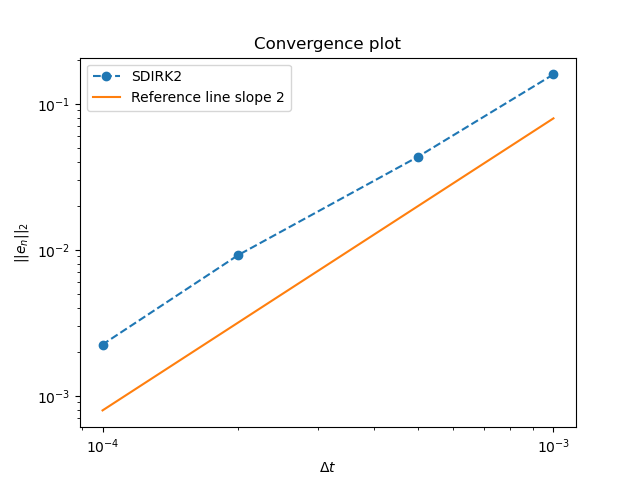
\includegraphics[width=\linewidth]{convergence.png}
	\caption{\label{normal_params} $\lambda = 1$ and $\alpha = 1$ in all rooms.}
	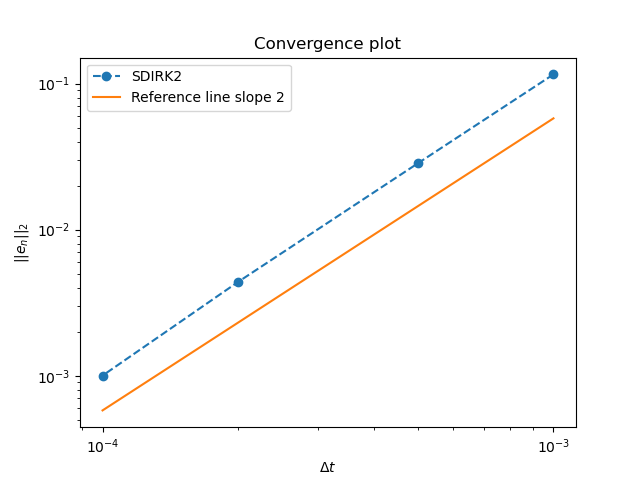
\includegraphics[width=\linewidth]{convergence_odd_params.png}
	\caption{\label{odd_params} $\lambda = 0.0243$ and $\alpha = 1300$ in $\Gamma_2$.}
\end{figure}

\begin{figure}
	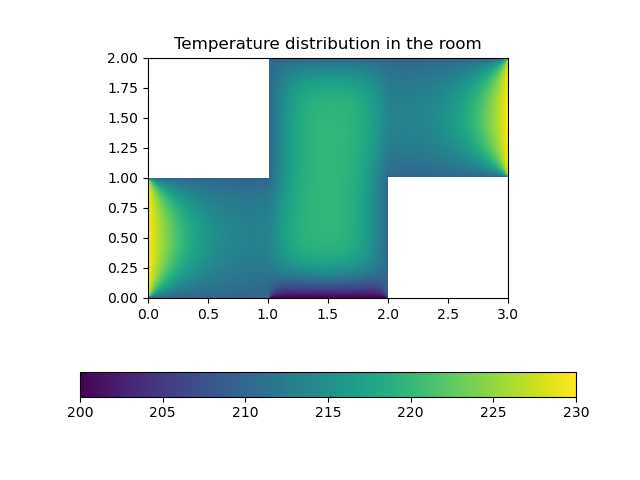
\includegraphics[width=\linewidth]{room_odd_params_1000}
	\caption{\label{room_odd_params_1000} $T=1000$, transient state.
	$\lambda = 0.0243$ and $\alpha = 1300$ in $\Gamma_2$.}
	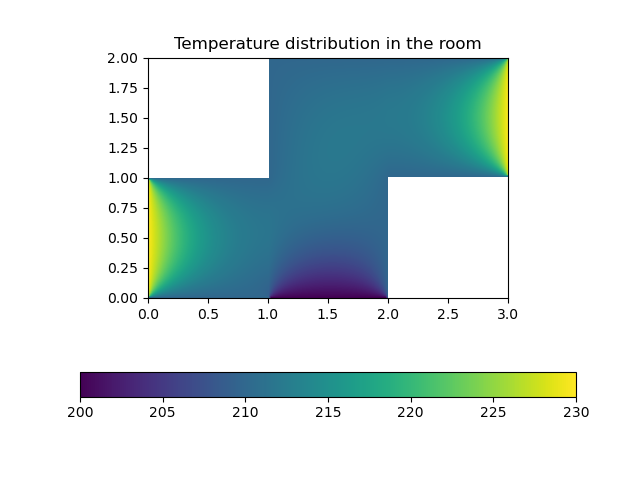
\includegraphics[width=\linewidth]{room_odd_params_10000}
	\caption{\label{room_odd_params_10000} $T=10000$, near steady state. $\lambda = 0.0243$ and $\alpha = 1300$ in $\Gamma_2$.}
\end{figure}
\begin{figure}

\end{figure}


\bibliographystyle{amsplain}
\bibliography{bib}





\end{document}
